\section{New design guide}
As Xamarin was changed to flutter, the entire frontend had to be reworked. 
Therefore we took a look at the old design guide and decided that there were things that we wanted to changed in order to get a more modern and simple design.
This meant that a new design guide had to be created.
The first thing we wanted to do was make the design guide more compact.
The old design guide was an 80 pages long pdf file that could be downloaded from Phabricator.
The new design guide is instead found on the GitHub wiki alongside the rest of the GIRAF project, making it is easier to find the guide and find the sections that a developer would need.
As seen on \autoref{fig:designguides}, the new one has fewer options, whereas the old one had 4 pages of content in the PDF file.
The reason that the new design guide is so much smaller, is mostly that a lot of the content in the old guide was talking about Android Studio specific implementation details, which is not relevant for the project development in Flutter, as it natively encourages following the material design guidelines.
However, the new design guide will most likely grow larger as the project goes on, but this should be an easy task for future students now that it is available as markdown files rather than a pdf document without any source available. 

\begin{figure}[H]
    \begin{subfigure}{0.6\textwidth}
    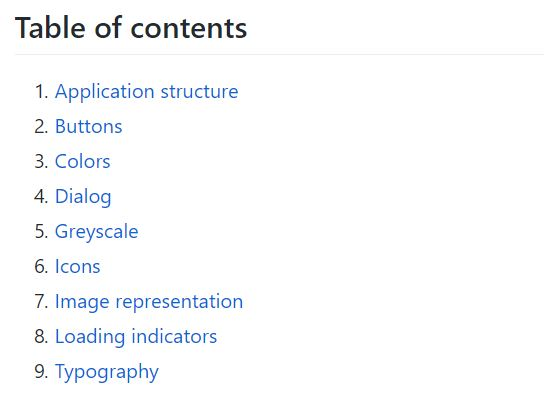
\includegraphics[width=1\linewidth, height=5cm]{figures/table-of-content-designguide.JPG}
    \caption{New design guide table of content}
    \label{fig:new-designguide}
    \end{subfigure}
    \begin{subfigure}{0.6\textwidth}
        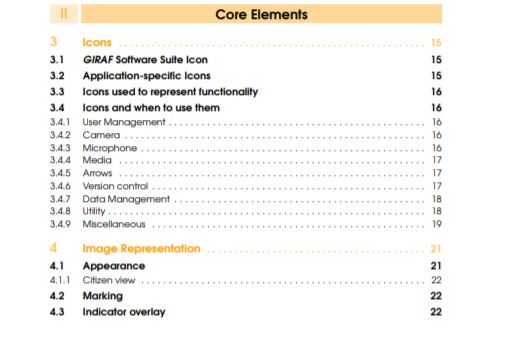
\includegraphics[width=1\linewidth, height=5cm]{figures/old-design-guide}
    \caption{Part of old design guide contents. Continues for another 3 pages}
    \label{fig:old-designguide}
    \end{subfigure} 
    \caption{New and old design guide.}
    \label{fig:designguides}
\end{figure} 

\subsubsection{Colors}
For the colors in GIRAF not much has changed from the old design guide to the new one. 
The only thing that changed was the colors for the weekdays.
The new colors are more dull compared to the old colors, giving a more subdued look with a more gentle impression.

\subsubsection{Typography}
The standard text color for typography is black.
The font was changed to \textit{Quicksand font}, because the customers prefer the letter "a" to be the handwritten version which this font allows.
The size of the font is 30 pt in landscape mode and in portrait mode it is 20 pt.
The text should also never be bold, italic or underlined to ensure consistent design.

\subsubsection{Icons}
Every icon in the old design guide has been changed for the new design guide.
The old icons had an out of date look, and did not result in a good design for the application.
Most of the icons that are used in this project are icons from the \textit{Font Awesome} project, which is a font and CSS framework.
These are easy to import in \texttt{Flutter}, and by using the icons in the same package the application is more consistent and will give the users a better experience, as they know the icons throughout the program.
Three custom icons needed to be created. \\
These can be seen on \autoref{fig:change-profile-icons}. \\\\
These icons are used for switching from guardian to citizen and vice versa and a new add timer icon.
In the old design guide there was only one icon for switching between guardian and citizen.
We wanted to make it more obvious which mode the user is in and decided to have two icons, one for each switch.
Depending on the mode the user is in the corresponding silhouette is colored in green.

\begin{figure}[htp]

    \centering
    
\includegraphics[width=.1\textwidth]{figures/changeToGuardian}\hfill
    
\includegraphics[width=.1\textwidth]{figures/changeToCitizen}\hfill
    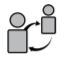
\includegraphics[width=.1\textwidth]{figures/old-change-profile}
    
    \caption{The rightmost picture is the old icon for changing profile. The middle is the icon to change from guardian to citizen and the leftmost is to change from citizen to guardian.}
    \label{fig:change-profile-icons}
\end{figure}


